\documentclass[Rapport/Rapport_main.tex]{subfiles}
\begin{document}
\section{RPiApp}
I denne sektion af rapporten vil de væsentligste dele af RPiApp blive forklaret. Applikationen kan opdeles i fire dele: Arkitekturen for designet og GameController klassen beskrives. Der beskrives softwaren for kernalspace driveren og til sidst boundary klasserne WebPage og Display.
\subsection{RPiApp - GameController}
I dette afsnit fokuseres på softwarens arkitektur, trådkommunikation og logiske operationer - Alle klasser i systemet har en relation til GameController klassen i form af MsgQueue kommunikationen, som er en klasse taget fra OS Api biblioteket udleveret i ISU\autocite{MSGQUEUE}.
\subsubsection{Softwaredesign}
\textbf{Event Dreven Arkitektur:} \\
Beer Pong er et eventbaseret spil. Det omhandler masser af asynkrone handlinger; når der rammes ned i en kop, fjernelse af kop, indsættelse af mønt mm. Det er således utrolig vigtigt, at vores system kan opfange alle disse asynkrone events. Selvom alle handlingerne fra brugeren er asynkrone, ønskes stadigt at interagere med handlingerne sekventielt. Dette er en vigtig faktor, for hvis en bruger laver to eventhandlinger inden for en kort tidsramme, skal der sikres, at systemet når at reagere på begge handlinger. En af måderne for at opnå dette er reaktiv programmering: Der ønskes at opdatere systemet med det samme, brugeren interagerer med det. \\
Dette problem løses ved event dreven arkitektur: Et system som reagerer ud fra signaler og tilstande fra aktører/delsystemer. Det er essentielt, at de asynkrone signaler afvikles sekventiel og i et trådsikkert system. Her anvendes klassen MsgQueue, som er baseret på Producer / Consumer idiomet.\autocite{Wiki_prod}
\begin{figure}[H]
    \centering
    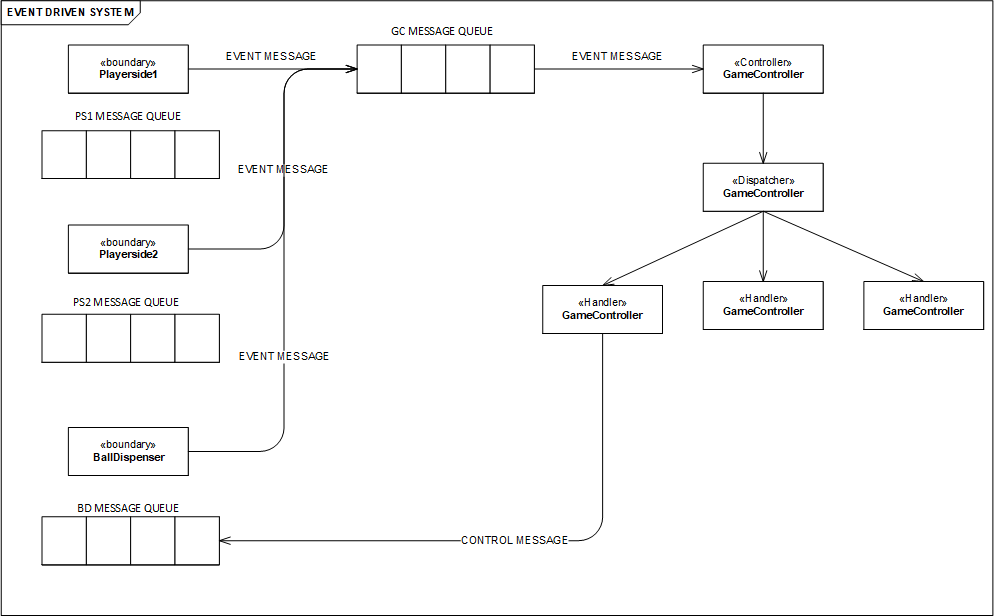
\includegraphics[width=1\textwidth]{Softwaredesign/RPiApp/graphic_RPi/EDS.png}
    \caption{Skitse af event driven system og MsgQueue system. Hvert boundary klasse har en MsgQueue instans, som er en 'consumer'. De andre klasser, som har tilgang til MsgQueue instansen, kan sende beskeder ved at allokere beskeder. Beskeden består af et id og en instans nedarvet fra klassen 'Message'. Som det kan ses på skitsen, er der ingen klasser, som har direkte 'kontakt' med hinanden, alt kommunikation sker gennem MsgQueues.}
   \label{fig:Sketch_Event}
\end{figure}
MsgQueue-systemet indfører også et trådsikret system, da alt data sendt gennem MsgQueue instanserne er indkapslet af mutex'er. Desuden allokeres og deallokeres nedarvede beskeder af base klassen Message dynamisk - denne form for hukommelsesadministration sikrer, at ressourcerne bliver frigivet korrekt, og der ikke opstår 'resource leaks'.\autocite{Resource}. For en mere detaljeret beskrivelse af event dreven arkitektur, håndtering af ressourcer og design overvejelser henvises til bilag \textbf{Software Design} afsnit \fullref{swdesign:sec:EventDriven}, samt afsnit \fullref{swdesign:sec:metode} for klassernes metodebeskrivelse.
\begin{figure}[H]
    \centering
    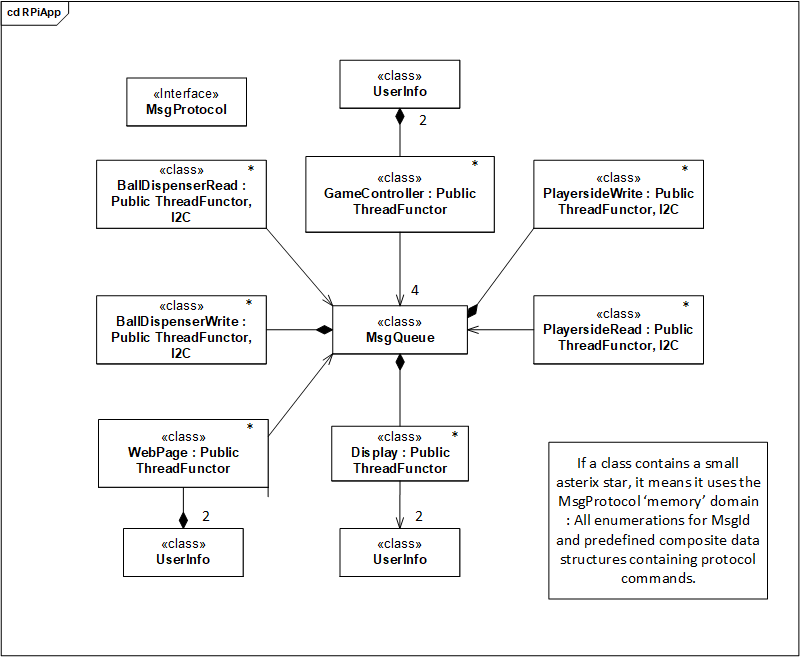
\includegraphics[width=1\textwidth]{Rapport/RPi/graphics/cd_RPiApp.png}
    \caption{Klasse diagram for RPiApp}
   \label{fig:cd_RPiApp}
\end{figure}
\textbf{RPiApp - GameController:}\\
Softwaredesignet for GameController, Playerside, BallDispenser, I2C og UserInfo er dokumenteret i afsnit \fullref{swdesign:sec:class_labels} i bilaget "Softwaredesign". \\
Controller klassen, GameController, beskrives kort i dette afsnit, da den er essentiel for hele systemet. \\
RPiApp er omfangsrigt program, og mange asynkrone handlinger og signaler skal behandles. GameController klassen er samlingspunktet for hele applikationen og indeholder alle de logiske operationer omhandlende spillet. Den bruger boundary klasserne til at dirigere PSoC-enhederne og Display. 
\begin{figure}[H]
    \centering
    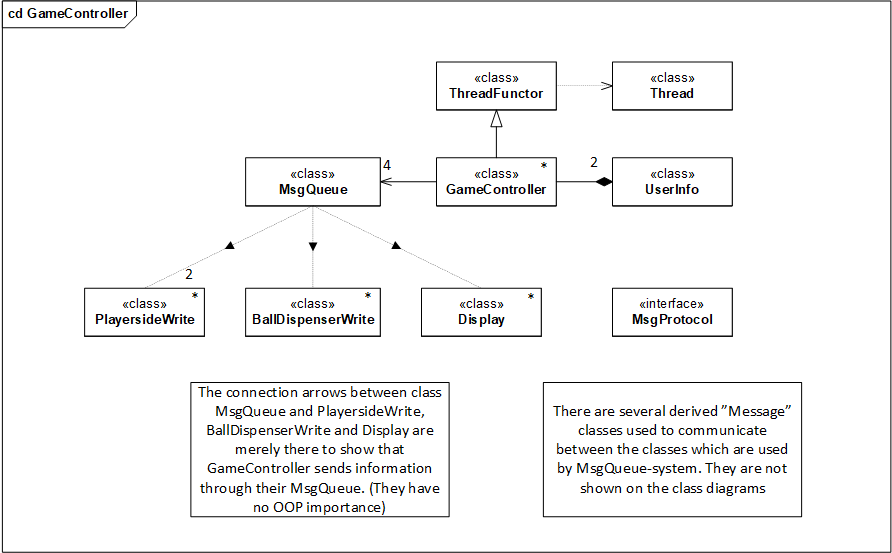
\includegraphics[width=1\textwidth]{Rapport/RPi/graphics/GameController.png}
    \caption{Klassediagram for GameController. GameController anvender MsgQueue associationerne til at kommunikere med boundary klasserne. Boundary klasserne viderefører alle kommandoer udsendt fra GameController videre til delsystemerne som Playerside og BallDispenser enhederne.}
   \label{fig:cd_GameController}
\end{figure}

\subsubsection{Implementering}
Softwareapplikation RPiApp er generelt udviklet objektorienteret i sproget C++. Sproget bruges, da det kan kompileres og afvikles på den valgte computerenhed, Rasberry Pi W Zero. C++ bruges til at udvikle det event driven arkitektur og det trådsikre system, men der bruges også elementer af C til at få adgang til filoperationer i kernelspace.

RPiApp's kildekode kan findes i bilaget \textbf{Kildekode}.

\subsubsection{Modultest}
Til test af GameController systemet blev white-box testing benyttet. Her blev de interne strukturer testet, primært MsgQueue trådkommunikationen. Trådkommunikationen blev testet ved at sende dynamisk allokeret beskeder mellem klasserne. \\
Black-box testning blev også brugt til at teste grænsefladerne for de øvrige delsystemer: Playerside-enhederne og BallDispenser-enheden. Grænsefladen til begge enheder består af I2C kommunikation. Da det ikke er muligt at få adgang til kernelspace operationer fra User Space uden driveren, blev filoperationerne blot testet. \\
Begge tests er nærmere beskrevet i afsnittet \fullref{modultest:sec:test_Game} i bilaget \textbf{Modultest}
\newpage
\subsection{RPiApp - WebPage}
Dette afsnit omhandler boundary klassen WebPage. WebPage er i denne forbindelse anvendt som en samlet betegnelse for alt, hvad der har med hjemmesiden at gøre. I virkeligheden består den af en klientside og en serverside, som kommunikerer internt gennem et WebSocket API. Et klassediagram for WebPage er vist i figur \ref{fig:WebPage_class_diagram}.

\subsubsection{Softwaredesign}
\begin{figure}[H]
    \centering
    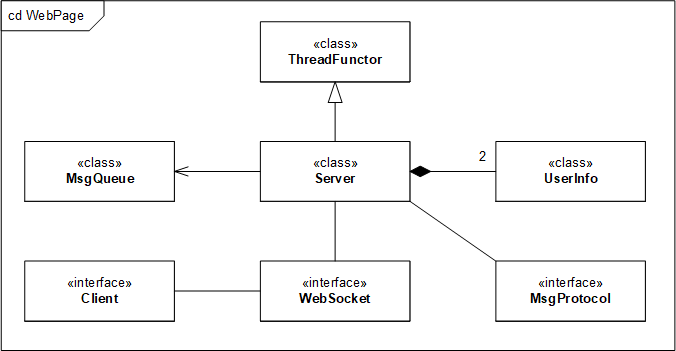
\includegraphics[width=1\textwidth]{Softwaredesign/RPiApp/graphic_RPi/cd_WebPage.png}
    \caption{Klassediagram for WebPage. Client anvendes som betegnelse for den side, der vises i webbrowseren. Server anvendes som betegnelse for den C++ klasse, som skal modtage brugerdata fra Client og videresende disse.}
    \label{fig:WebPage_class_diagram}
\end{figure}

\textbf{Websocket}
\\Webkommunikation forløber typisk ved, at der etableres et forhold mellem client og server, som er baseret på anmodninger og svar. Client kan eksempelvis være en webbrowser og server en applikation, som hoster en hjemmeside. En ofte anvendt protokol til denne form for kommunikation er HTTP.\cite{http_wiki} Ved at opdatere HTTP-forbindelsen til en WebSocket kan der etableres en vedvarende forbindelse mellem client og server. Kommunikationen kan dermed betegnes som full-duplex.\cite{websocket_wiki}\\
\newline
\textbf{Client}\\
Client beskriver hjemmesidens interface. Det er her defineret, hvordan hjemmesiden skal præsentere sig i webbrowseren. Under initieringen af siden oprettes WebSocket objektet, og de event handlers som er en del af API er ligeledes implementeret her. Når data skal sendes mellem Client og Server, skal det ske i tekstformat. Der er derfor designet en løsning, hvor spillerne har mulighed for at indtaste holdnavne og brugernavne samt vælge holdfarver på track bars for henholdsvis hold 1 og hold 2. Når der trykkes på en 'Start' knap på hjemmesiden, genereres et event, som medfører, at alle brugerinputs konkateneres til én tekststreng og sendes til Server.\\
\newline
\textbf{Server}\\
Serversiden har til opgave at modtage og behandle førnævnte data fra Client. Den lytter aktivt på den relevante port, og når tekststrengen modtages bliver denne indlæst i en buffer og separeret på passende vis. Informationerne opbevares i STL Vector og anvendes til at sætte members på to objekter af UserInfo klassen, team1\_ og team2\_. Disse objekter skal sendes til GameController klassen, og hertil anvendes det tidligere beskrevne event drevne system med Messages og MsgQueues. WebPage har derfor kendskab til GameControllers MsgQueue, men det omvendte gør sig ikke gældende. Der forudses problemer med race conditions, og kommunikationen mellem server og GameController er derfor bevidst gjort envejs.\\WebPage er opsummeret i et sekvensdiagram i figur \ref{fig:WebPage_sequence_diagram}. Flere detaljer om designet kan ses i afsnit \fullref{swdesign:sec:webpage_doc} i bilaget \textbf{Softwaredesign.}
\begin{figure}[H]
    \centering
    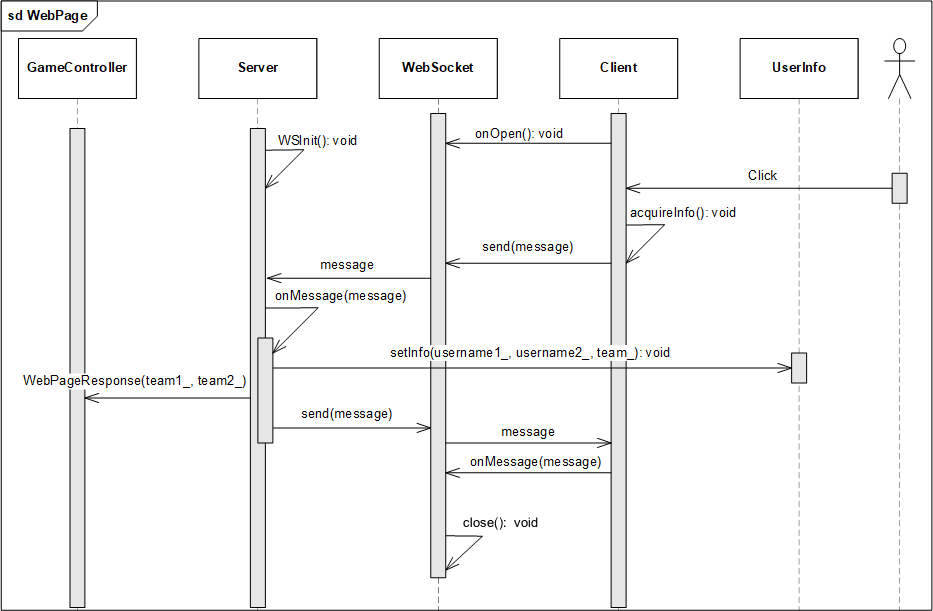
\includegraphics[width=1\textwidth]{Softwaredesign/RPiApp/graphic_RPi/WebPage_sd_2.png}
    \caption{Sekvensdiagram for WebPage. Det viser, hvordan Client og Server kommunikerer internt gennem et WebSocket API, og at sidstnævne sender \textit{\textbf{spiller oplysninger}} til GameControllers MsgQueue}
    \label{fig:WebPage_sequence_diagram}
\end{figure}
\subsubsection{Implementering}
Webserver afvikles af en RPi Zero W. Den er derfor implementeret som en C++ klasse. Hjemmesidens interface beskrevet i afsnittet \textbf{Client} er implementeret med det såkaldte 'markup language' HTML5 i kombination med Cascading Style Sheets (CSS). Script-sproget Javascript anvendes til at implementere hjemmesidens dynamiske elementer samt WebSocket API. Den valgte løsning tager udgangspunkt i slides\cite{websockets_getting_started}. Der anvendes open-source biblioteket uwebsockets\cite{uwebsockets_repo} og visse elementer fra de eksempler, som blev præsenteret i slides. For flere informationer vedrørende implementeringen henvises til afsnittet \fullref{swdesign:sec:webpage_implementering} i bilaget \textbf{Softwaredesign.}

\subsubsection{Modultest}
De vigtigste krav for WebPage er opsummeret  nedenfor.
\begin{itemize}
    \item Alt tekst på WebPage skal være på sproget engelsk
    \item På WebPage skal der for hvert af de to hold indtastes følgende \textit{\textbf{spiller oplysninger}}: \textit{teamname}, \textit{username1} og \textit{username2}
    \item Holdnavne og brugernavne indtastet på WebPage skal være tekststrenge, med en længde på mellem 1 og 15 karakterer
    \item På WebPage skal der for hvert af de to hold kunne vælges følgende \textit{\textbf{spiller oplysninger:}} \textit{holdfarve}, ved at justere intensiteten af farverne rød, grøn og blå i et RGB farveskema.
    \item Der skal kunne vælges mindst 10 forskellige farver på WebPage.
\end{itemize}
For at teste kravene er der lavet et testprogram, som udskriver \textit{\textbf{spiller oplysninger}} i terminalen i ubuntu, hver gang data sendes fra Client til Server. Testen foretages ved at indtaste \textit{\textbf{spiller oplysninger}} på hjemmesiden, trykke 'Start' og herefter undersøge terminal output. Dette gentages 50 gange, mens navne og farver varieres, og resultatet fremgår af tabellen nedenfor.
\begin{table}[H]
    \centering
    \begin{tabular}{|L{0.15\textwidth}|L{0.15\textwidth}|L{0.15\textwidth}|}
         \hline
         \textbf{Forsøg, n} & \textbf{Korrekt output} & \textbf{Fejl} \\ \hline
         50 & 50 & 0 \\ \hline 
    \end{tabular}
    \caption{Data sendes fra client til server 50 gange}
     \label{tab:webpage_data_2}
\end{table}
Hjemmesiden er vist i browseren i figur \ref{fig:webpage_modultest_rapport_1}, mens det resulterende terminal output fremgår af figur \ref{fig:webpage_modultest_rapport_2}.
\begin{figure}[H]
    \centering
    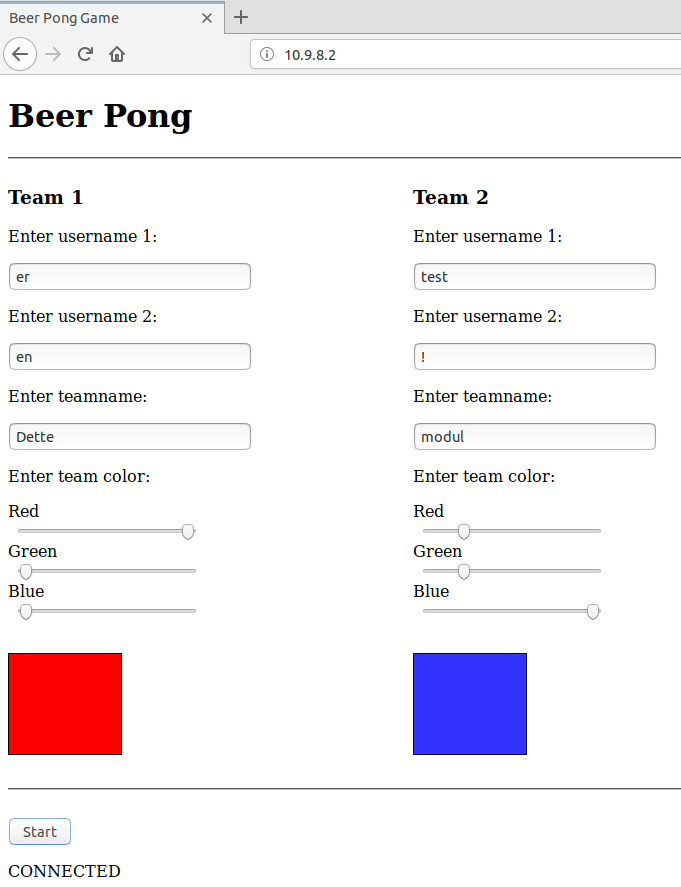
\includegraphics[width=0.6\textwidth]{Modultest/WebPage/graphics/modultest_1.png}
    \caption{Modultest - hjemmeside vist i browser}
    \label{fig:webpage_modultest_rapport_1}
\end{figure}
\begin{figure}[H]
    \centering
    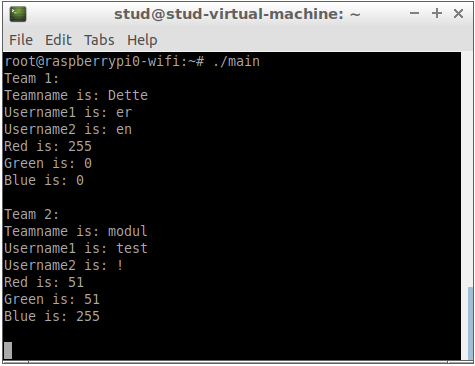
\includegraphics[width=0.5\textwidth]{Modultest/WebPage/graphics/modultest_2.png}
    \caption{Modultest - terminal output}
    \label{fig:webpage_modultest_rapport_2}
\end{figure}
Ved visuel inspektion af hjemmesiden i figur \ref{fig:webpage_modultest_rapport_1} kan det konkluderes, at kravene angivet ovenfor er opfyldt. Desuden virker det til, at \textit{\textbf{spiller oplysninger}} sendes korrekt fra Client til Server. For yderligere informationer vedrørende modultesten henvises til afsnittet \fullref{modultest:sec:webpage_modultest} i bilaget \textbf{Modultest}.

\subsection{I2C\_interruptDriver}
\subfile{Rapport/RPi/I2C_interruptDriver/Design.tex}
\subfile{Rapport/RPi/I2C_interruptDriver/Implementering.tex}
\subfile{Rapport/RPi/I2C_interruptDriver/Modultest.tex}




\subsection{RPiApp - GUI}
\subsubsection{Softwaredesign}
\textbf{Display design}
\begin{figure}[H]
    \centering
    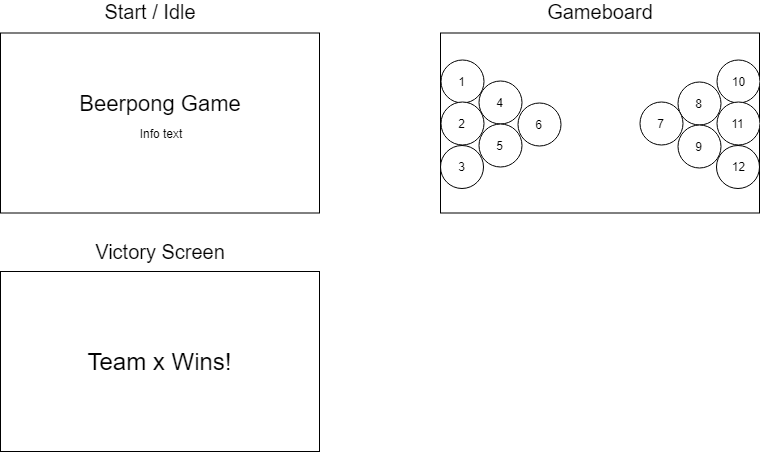
\includegraphics[scale=0.5]{Softwaredesign/GUI/Pictures/Boards.png}
    \caption{Forskellige design af "Game boards". Der ses: en IDLE state,  En Gameboard state,  en Victory screen og en Service screen. Hvad der definerer en "state" er,  at  de har en unik baggrund. Det vil sige at teksten vist på skærmen, fx. holdnavne, ikke ændrer på hvilken state, man befinder sig i.  }
    \label{gameboards}
\end{figure}

På figur \ref{gameboards} kan ses forskellige states, som displayet kan vise.  Der er et ''Start/Idle'' state. Dette er det state, som displayet vil vise, når der intet spil er igangværende. Gamboard state er det state, som er aktivt, når et spil er igangværende. Victory screen er det state, som aktiveres, når et hold rammer den sidste kop, og spillet er vundet. Service state er det state, som er aktivt, hvis der er mindre end to bolde tilbage i \textbf{Balldispenser}. \\
Måden der skiftes mellem states er via. beskeder fra en message queue; for at se mere omkring message queue se afsnit \fullref{swdesign:sec:display_q_doc}. De beskeder håndteres så af en af masse ''handler funktioner'', som styrer, hvad der vises på skærmen; for mere omkring de omtalte handlers se afsnit \fullref{swdesign:sec:GUI_funktionsbeskrivelse_doc} i bilag \textbf{Softwaredesign}.\\
Der laves et Statemachine diagram på figur \ref{GuiDisplayStatemachine}, som viser sammenhængen mellem de tilgængelig states og de omtalte handlers.


\begin{figure}[H]
    \centering
    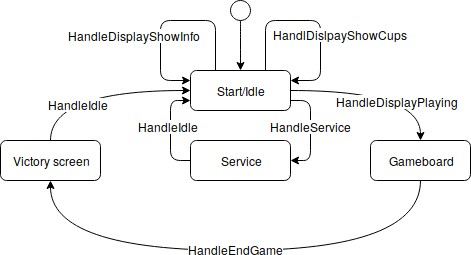
\includegraphics[scale=0.8]{Softwaredesign/GUI/Pictures/Gui_displaystatemachine.png}
    \caption{Statemachine for display tilstand}
    \label{GuiDisplayStatemachine}
\end{figure}

%----------------------------------------------------------------------

\textbf{Display layout}
\begin{figure}[H]
    \centering
    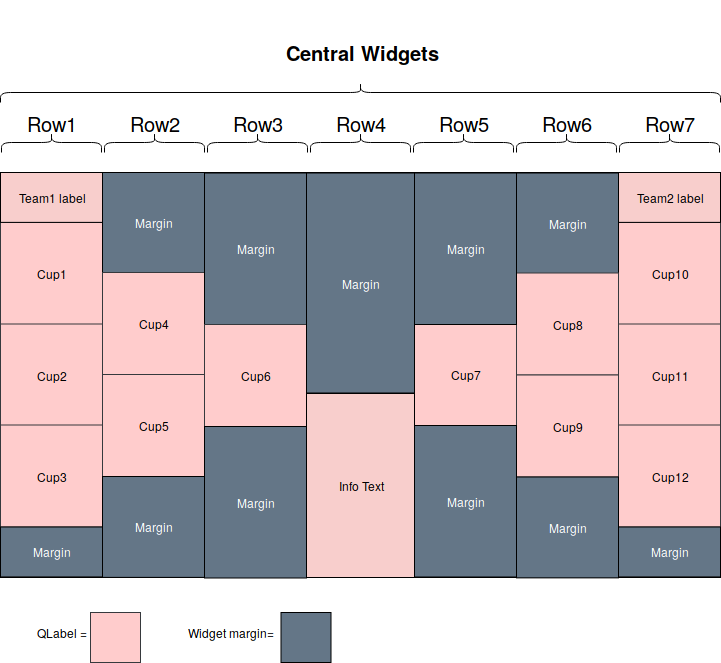
\includegraphics[scale=0.5]{Softwaredesign/GUI/Pictures/Boards_design.png}
    \caption{Visualisering af implementering GUI Widgets og Labels. Der vises Label (Typen QLabel), denne type er i stand til at vise BÅDE tekst og billeder. Margin er en tom plads, som ikke bliver brugt.    }
    \label{gui_design_implementering}
\end{figure}
GUI'en har et fast layout. Dette betyder, at labels, widgets osv. ikke bevæger sig i forhold til hinanden. Det har fordelen, at applikationen vil passe til flere forskellige skærmopløsninger eller vinduesstørrelser. Dette faste layout opnås ved at først at ''definere'' hele programmet; i dette tilfælde ville hele programmet være ''Centrel Widget''. Central widget ville være der, hvor baggrunden ville vises på. Det centrale widget deles derefter op i 7 rækker: Row1-Row7. Derudover indeholder rækkerne også Labels. Alle rækkerne er delt op i kolonner. I disse kolonner bestemmes størrelsen af ''Margin'', ellers bestemmes størrelsen af QLabels. Det ses på figur \ref{gui_design_implementering}, hvad hver QLabel bliver brugt til når i brug. Cup1 til og med Cup12 bruges til at vise, om en given kop er ''on'' eller ''off''. Ellers er der et QLabel, som bruges til ''info text'' som er tekst, som anviser hvad brugeren skal gøre for at starte spillet. Team1 og Team2 labels indeholder: holdnavne og brugernavne. Alle disse labels er nødvendigvis ikke synlige, men skal altid logisk gemmes i hukommelsen.

\subsubsection{Implementering}
GUI er implementeret i form af en UI QT design fil,  en C++  klasse samt en qrc ressource fil. UI-filen står for selve udseendet af GUI'en; hvor at C++ klassen står for opførslen af GUI'en. qrc ressourcefilen er en fil, som bruges til at tilgå de forskellige billeder, som bruges i GUI'en. For mere info se afsnit \fullref{swdesign:sec:GUI_implementering_doc}
\subsubsection{Modultest}

\textbf{Display Modultest}\\
I modultest af display delen af RPi-applikationen blev det testet:  Kan display applikationen fungere på en 24 tommer skærm, med en 1920x1080 opløsning? Kan display applikationen modtage beskeder fra message queue systemet? Håndterer display applikationen som ønsket på baggrund af beskeder modtaget fra message queue. For en fyldestgørende gennemgang af modultest , se afsnit \fullref{modultest:sec:GUI_modultest_doc} i bilag \textbf{Modultest}

\textbf{Opsummering}\\
På baggrund af overnævnte krav til displayet gennemførte Display delen af RPi-applikationen  modultesten.
\end{document} 